\chapter{Identifikáció}\label{chap:ident}


A szabályzó tervezésénél használt szakaszmodell (gerjesztés-válasz kapcsolat) a Simulinkben megvalósított fizikai modell viselkedését leíró rendszer átviteli függvénye lesz. A Simulinkben vizsgálójeleket használok: a több bemenetű, egy kimenetű rendszert egyszerre csak egy bemenetén gerjesztem (\textit{\ref{fig:valve-step}. ábra}). 
% a kimeneti változást létrehozó hatás egyértelműen beazonosítható kell hogy legyen.

\begin{figure}[H]
	\centering
	% trim={<left> <lower> <right> <upper>}
	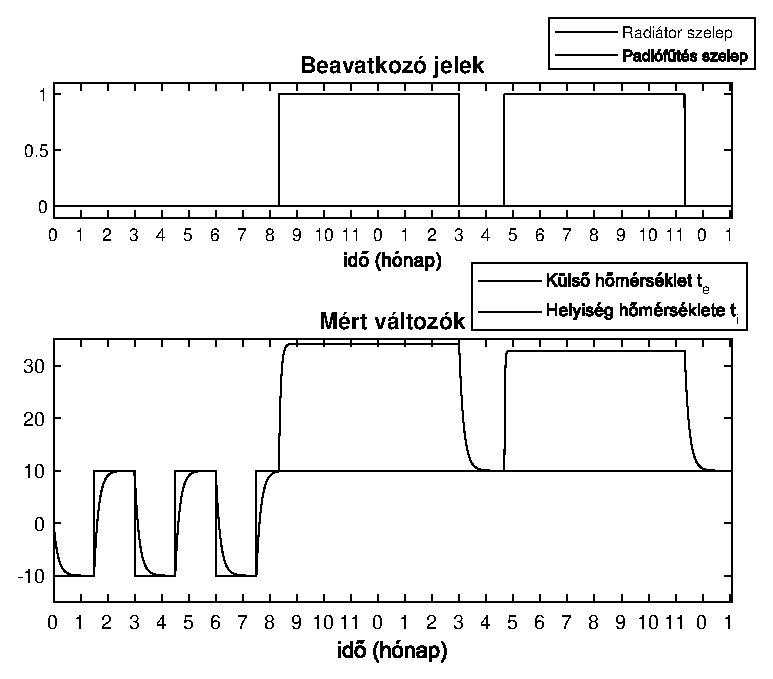
\includegraphics[trim=0 0 0 0, clip,width=0.9\textwidth]{figures/valve-step}
	\caption{Szimulációs eredmények a bemeneteket külön-külön gerjesztve}
	\label{fig:valve-step}
\end{figure}

A módszer az, amit a több forrást tartalmazó hálózatok esetén is alkalmazunk: a válasz számításakor mindig egy forrás hatását vizsgáltuk, a többit dezaktivizáltuk: azaz a több bemenetű Simulink hálózatnak egyszerre csak egy bemenetét gerjesztem. Lineáris hálózat vizsgálatakor a kimeneten a válasz szuperpozícióval adódik. 

\begin{figure}[H]
	\centering
	% trim={<left> <lower> <right> <upper>}
	\includegraphics[trim=0 0 0 0, clip,width=0.9\textwidth]{figures/valve-nonlinearity}
	\caption{Szimulációs eredmények a szelepeket lépcsős függvénnyel gerjesztve}
	\label{fig:valve-stair}
\end{figure}



%A szuperpozíció módszere itt csak korlátozásokkal működik. A fűtőtestekben ugyanis adott hőmérsékletű víz kering, így ha a környezeti hőmérséklet megnő, azok teljesítménye lecsökken. 

A Simulink modellt bemenetein gerjesztem (külső hőmérséklet \SI{40}{\celsius}, majd fűtés \SI{60}{\celsius} előremenő hőmérsékleten valve = 1 állásban.\footnote{A stratégia lehet $t_s$ előremenő hőmérséklet vagy $\xi \cdot \dot m$ tömegáram szabályzása $\alpha$ = [0..1] beavatkozójellel. })



Az identifikációhoz adatfile-t hozok létre, a Simulinkben IDDATA blokk a be- és kimenetek értékét mintavételi időnként rögzíti és a \textit{Base Workspace}-be menti. Innen a \textit{System Identification} app-ba betölthetők az adatok. %A mintavételi idő először egy másodperc volt. %A Matlab Workspace-ben megjelenik egy iddata, ezt tudom az ident toolboxba importálni.
Erre átviteli függvényeket illesztek. Az átviteli függvények pólusainak, zérusainak a száma a Simscape modell alapján meghatározható, RC-hálózatok analógiájával.

Nyilvánvalóan célszerű az identifikációnál minél nagyobb változásokat mérni. Nem tartottam "értelmét" 1\si{\celsius}-os step jelre identifikálni. Így beállítottam nulla kezdeti értéket a ház összes paraméterére. (Falak, fűtési rendszer, stb. Nyilvánvaló, hogy ilyenkor nem a realizmus a cél, hiszen a nagy változásokra jön elő a rendszer dinamikája.) Nulla kezdeti értékből a környezeti hőmérsékletet 0-ról 40\si{\celsius}-ra emeltem, ennek a beállási ideje több nap volt, majd visszaállítva 0\si{\celsius}-ra megvártam a lecsengést, ezután pedig a beavatkozó szelepeket teljesen kinyitottam. 

Egy ilyen szimuláció a fenti szekvenciával kb. 50 napnyi viselkedést fog át, ez másodperces mintavételi idővel rengeteg adat, amivel meggyűlik az Ident Toolbox baja is.

5 perces mintavételi időkkel már sokkal gyorsabban lefut a Simulinkben a szimuláció és a toolboxban az identifikáció, lénygében azonos eredményt adva.

Viszont a mintavételi idők megváltoztatásánál, nem volt egyértelmű, hogyan reagál a Simscape vagy az MPC. A Simscape-nél kiderült, hogy a mintavételi időt manuálisan nem lehet megadni.


\begin{figure}[H]
	\centering
	% trim={<left> <lower> <right> <upper>}
	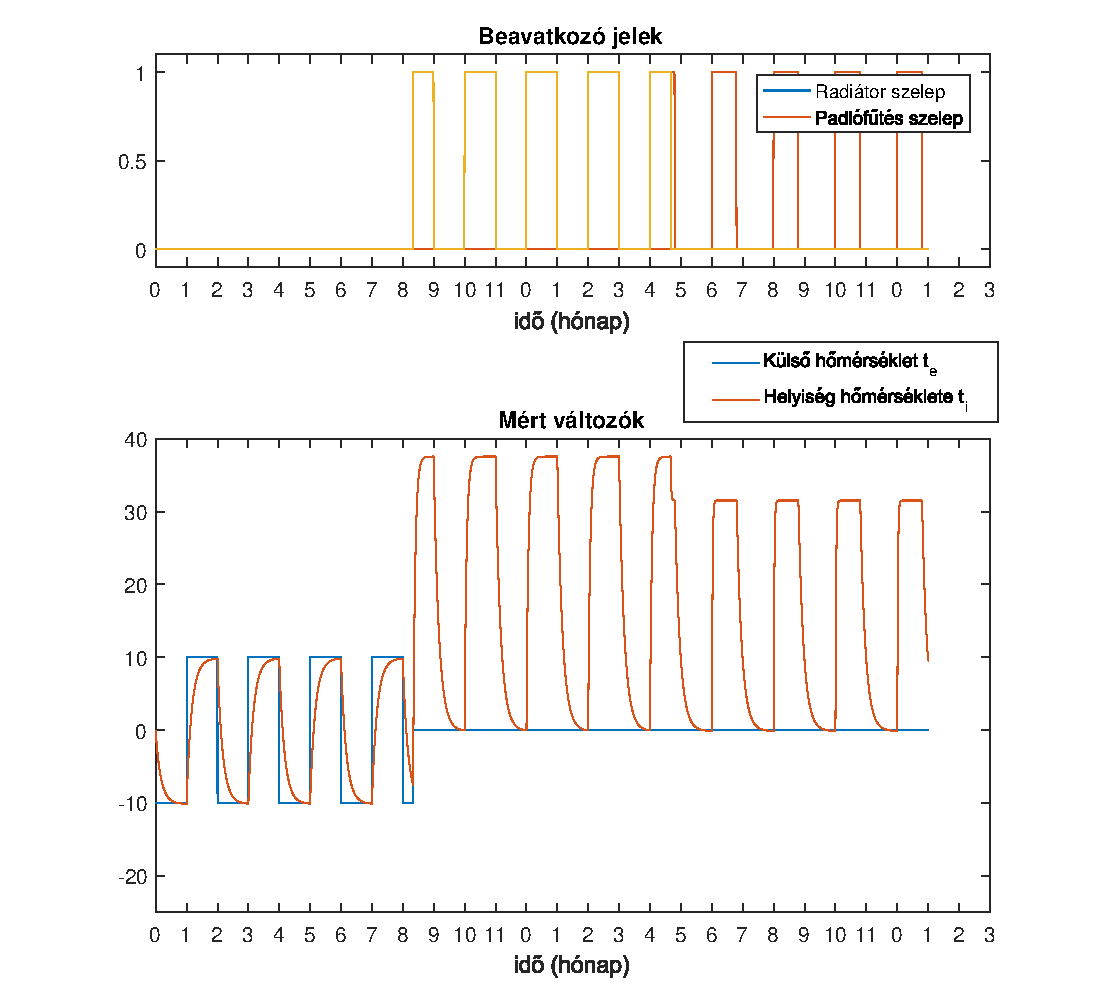
\includegraphics[trim=0 0 0 0, clip,width=\textwidth]{figures/ident-valve3}
	\caption{Identifikáció során }
	\label{fig:ident}
\end{figure}

Az identifikáció pontosságának javításához mindhárom bemeneti változó hatását több periódusra rögzítettem, 750 napnyi szimulációval. Ez fél órás mintavételi idő mellett szimulációban kevesebb, mint 1 perc alatt futott le\footnote{7. generációs i5 processzor, 8GB RAM, SSD használatával}. Az identifikációhoz a hőmérsékletet kelvinben rögzítem, mivel \si{\celsius} használata esetén az összefüggések nem lineárisak. (A kelvinben mért hőmérsékletet nevezik termodinamikai hőmérsékletnek.) A fenti esetben a beállási idők kb. 30 naposak az egész rendszert tekintve, ami kb. 10 napos időállandót jelent. Szakirodalom szerint a falszerkezetek időállandója kb. 5 nap, a helyiségre így reálisnak tűnik a közelítés.
%Zérusok hatása röviden. Mit tud. Hánytárolós rendszer. Néhány kép.
%MISO identifikáció. 
%
%
%\section{Hagyományos szabályzás performanciája}
%
%PI, miért nem jó
%Csak SISO-ra működik és itt esetünkben itt több bemenetről van szó mindenképpen. Irodalom: S. Prívara et al. 
%


\pagebreak